%!TEX root = maincl.tex
%
\clearpage
\appendix
\section{Appendix}

Accompanying the submission \textit{\titlename}.


\subsection{comments on features}
\verify{Feature sets construction problems (after investigating code):
\begin{itemize}
	\item Stance splitting different cutoffs for different features (.25 and .75 for \textbf{FS1} and \textbf{FS3}, but .1 and .9 for \textbf{FS2}). Twitter predictor gives prob of being pro-Brexit.
	\item When removing duplicates, it removes the "2", "2 2" and "2 2 2" (\textbf{FS1}, line 84). Also the distribution of classes does not match after the removal of duplicates.
	\item In \textbf{FS1}, it only uses the reported number of comments \textbf{per post/submission}, and they extend over all periods. In \textbf{FS2}, it reports comments \textbf{per entry (post or comment)}, and only during current time period;
	\item In \textbf{FS2}, when computing the emitted comments to others from stances, if the parent is not in current period (for example, the parent was in a different time period), it won't be found. Therefore $CS_t(u) \neq CS_t^{A}(u) + CS_t^{P}(u) + CS_t^{N}(u)$
	\item \textbf{FS2} also contains $ID_t(u)$ and $CS_t(u)$ from \textbf{FS1}, in the code.
	\item In \textbf{FS3}, only the comments and posts emitted during current period are considered when computing percentages.
\end{itemize}
}
\subsection{Prediction  for Neutral}

\cl{remove paragraph ci dessous ou a verifier -> Predicting the following stance}
Furthermore, in order to explain these results, we compute volume of users corresponding to each of the 9 transitions. The results are shown in \cref{tab:volume_users}. This table explains the values from \cref{fig:table_f1_scores}. Firstly, the number of users having a Neutral - Neutral trajectory is considerably small, because of the applied filtering, namely the removal of entries having translation Neutral - Neutral which appear only once, for a given set of input features. Next, we obtain very low scores for the transitions from a pro Brexit stance to an against Brexit stance and vice-versa because the number of examples of users in these situations is very small compared to the other categories, 35 and 33 respectively. 
%!TEX root = maincl.tex
%
% Please add the following required packages to your document preamble:
% \usepackage[table,xcdraw]{xcolor}
% If you use beamer only pass "xcolor=table" option, i.e. \documentclass[xcolor=table]{beamer}
\begin{table}[htp]
	\centering
	\caption{The volume of users in the testing set for each category of transitions.}
	\label{tab:volume_users}
	\begin{tabular}{ccc}
	\toprule
	\textbf{\begin{tabular}[c]{@{}c@{}}Current\\ Stance\end{tabular}} & \textbf{\begin{tabular}[c]{@{}c@{}}Following\\ Stance\end{tabular}} & \textbf{\begin{tabular}[c]{@{}c@{}}Number of\\ Users\end{tabular}} \\ \midrule
{\color[HTML]{FE0000} Against}                                    & {\color[HTML]{FE0000} Against}                                      & 158                                                                \\ 
{\color[HTML]{FE0000} Against}                                    & {\color[HTML]{3166FF} Brexit}                                       & 33                                                                 \\ 
{\color[HTML]{FE0000} Against}                                    & {\color[HTML]{656565} Neutral}                                      & 371                                                                \\
{\color[HTML]{3166FF} Brexit}                                     & {\color[HTML]{FE0000} Against}                                      & 35                                                                 \\ 
{\color[HTML]{3166FF} Brexit}                                     & {\color[HTML]{3166FF} Brexit}                                       & 60                                                                 \\
{\color[HTML]{3166FF} Brexit}                                     & {\color[HTML]{656565} Neutral}                                      & 332                                                                \\ 
{\color[HTML]{656565} Neutral}                                    & {\color[HTML]{FE0000} Against}                                      & 387                                                                \\ 
{\color[HTML]{656565} Neutral}                                    & {\color[HTML]{3166FF} Brexit}                                       & 350                                                                \\ 
{\color[HTML]{656565} Neutral}                                    & {\color[HTML]{656565} Neutral}                                      & 27                                                                 \\ \bottomrule
\end{tabular}
\end{table}

Indeed, the chances that a user will change his position in two consecutive time-frames from totally Brexit supporting to totally against Brexit are low and this is revealed by the distribution presented in \cref{tab:volume_users}.  In most situations, there will be a transition through the intermediate Neutral state, also shown by \cref{tab:volume_users}, the number of users going from Against and Brexit to Neutral being 371 and respectively 350. This allows our classifier to understand the underlying structure of the dataset, leading to high F1-scores for these translations.

\hl{The XGBoost classifier obtains an overall F1-score of 0.57, using the FS4 feature set. We can identify two main sub-components of this score: the first one is represented by the low scores obtained when predicting transitions Brexit - Against or Brexit - Brexit, which lowers the overall score. The second sub-component is defined by the predictions involving the Neutral state, namely from Neutral to the other three states.}

Predicting the following stance a user will arrive into turns out to be a difficult task, notably when the user changes of opinion. 
\cl{verifier figure envoye par mel le 8/05 Pbl}
In \cref{fig:figure_12} we show the volume of users translating from neutral state to a Brexit supporting state or Against Brexit state, in consecutive time-frames. The left figure shows the percentage of users, while the right figure shows the exact number of users going to the two polarized states. We can observe that except the starting time-frame, where there was a strong campaign for Brexit which is reflected in the ratio of users who migrated to a Brexit stance in the second time-frame, usually the trend is in favor of the Against side. In translations from T2 to T12, neutral users tended to move to Against Brexit. However, in T12, there is a change in the trend. 

\begin{figure*}[tbp]
	\centering
	\newcommand\myheightA{0.175} %% full size: 0.173
	\subfloat[]{
		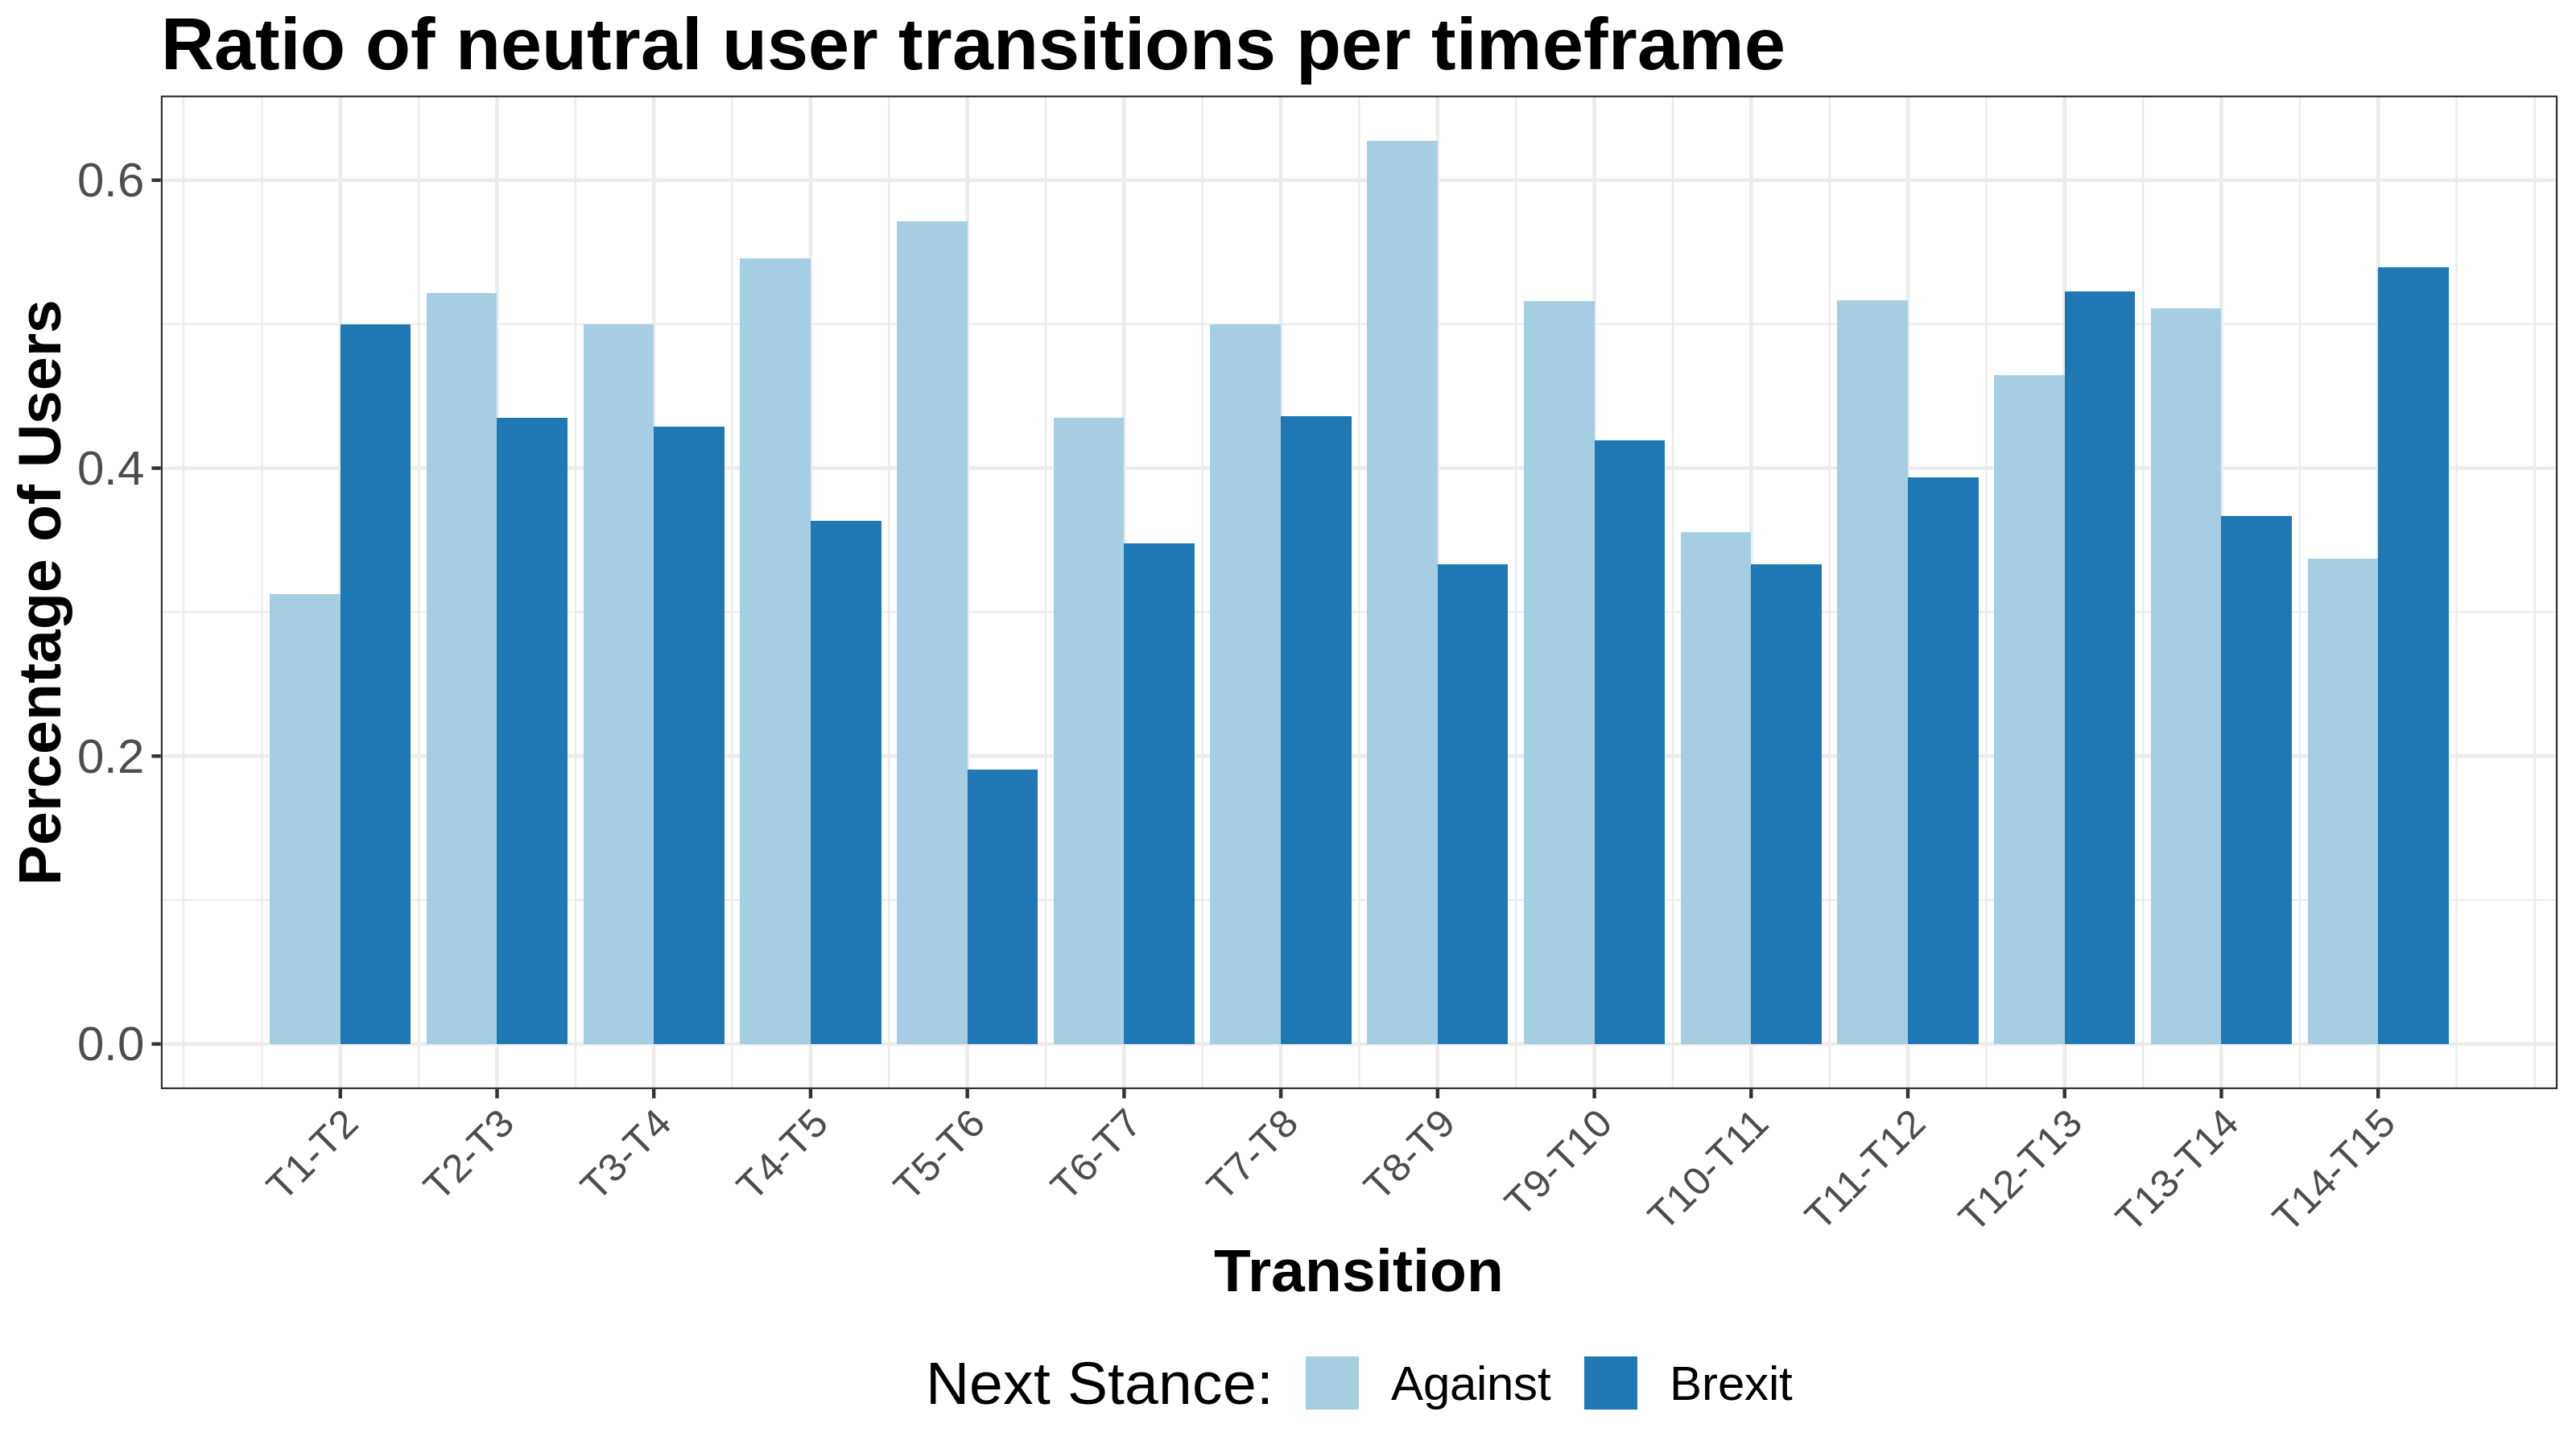
\includegraphics[height = \myheightA\textheight]{ratio_user_transitions}%
		\label{subfig:neutral-ratio}%
	}%
	\subfloat[]{
		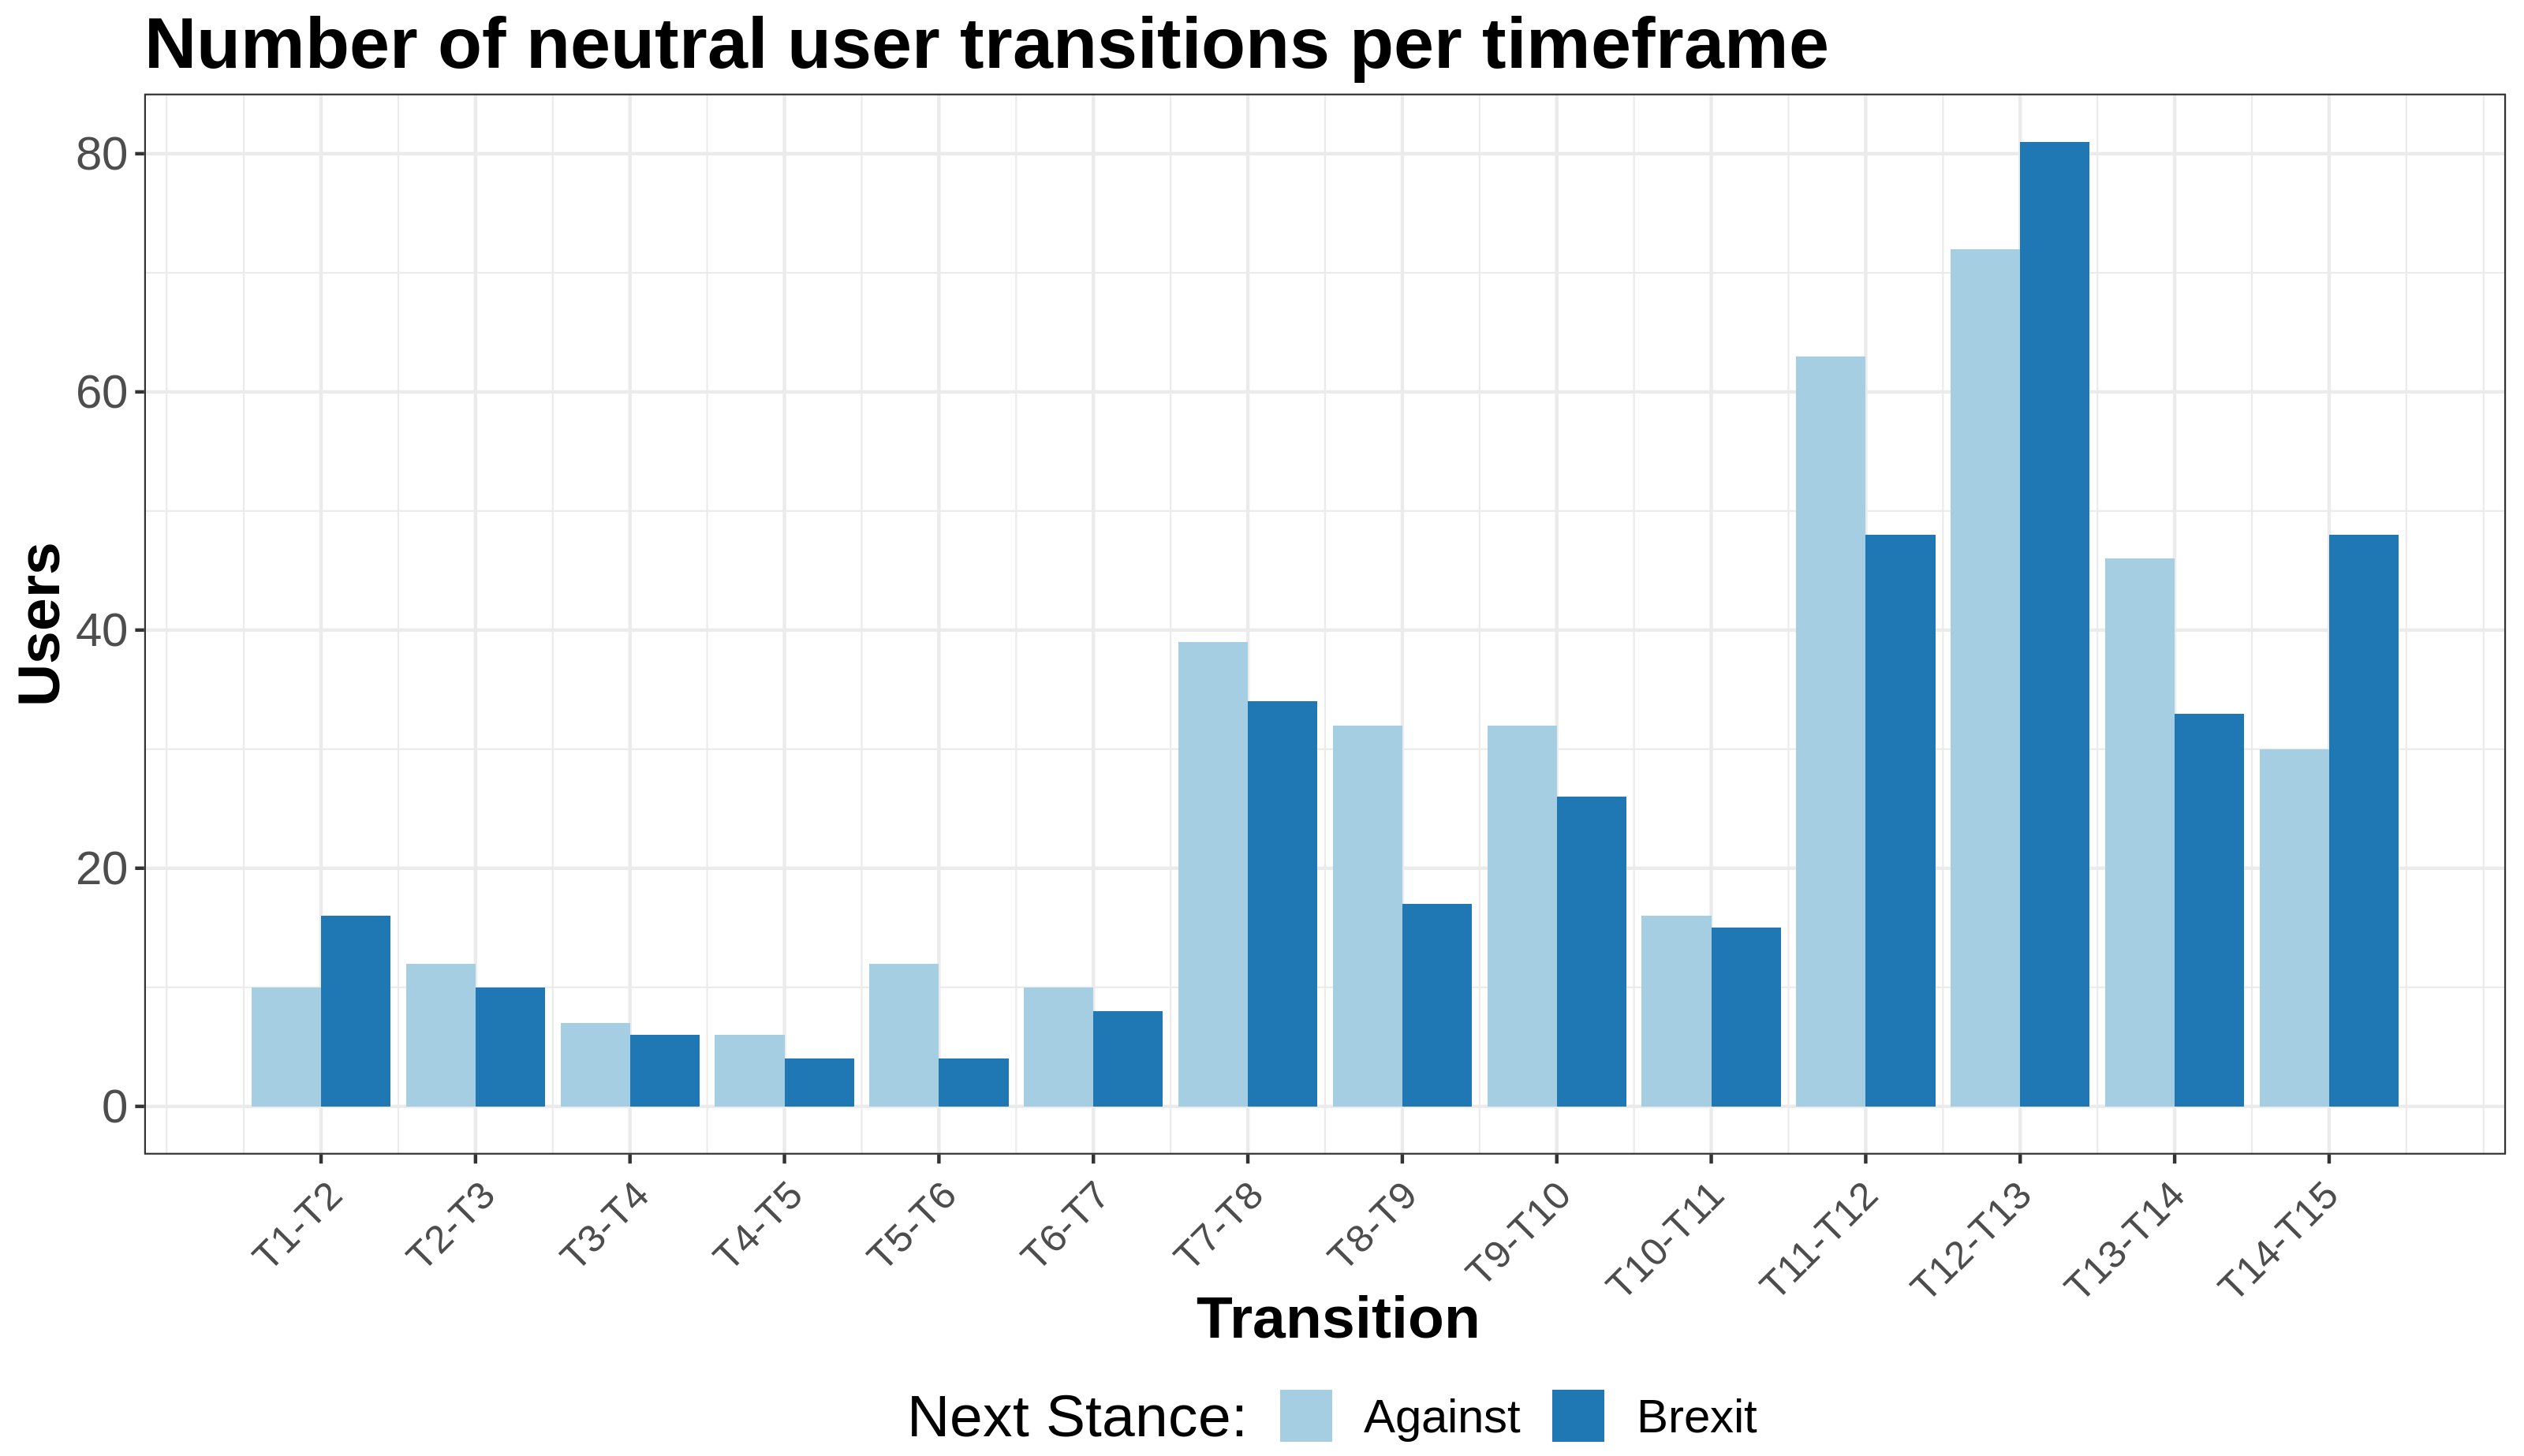
\includegraphics[height = \myheightA\textheight]{number_user_transitions}%
		\label{subfig:neutral-volume}%
	}%
	\caption{ 
		\TODO{MAR}{PDF (vectorial) version needed!}
		a) Ratio of users transitioning to the other stances in consecutive time-frames.  ratio. 
		b) Number of users transitioning to the other stances in consecutive time-frames. 
	}
	\label{fig:figure_12}
\end{figure*}

We performed some analysis on this period and found out that the main event in this period of time was the second negative vote in the Parliament for the Withdrawal Agreement negotiated by Theresa May. UK would have had to pay the European Union 39 billion pounds, which was upsetting and disappointing for people, as revealed by some of the utterances we checked (we checked utterances with high leave probability): "\textit{It's taken far too much time, we should leave hard and deal with the consequences. It will be tough for a time but there's no price not worth paying for freedom from the globalist overlords... ``It's **better** to **die free**, **than live** as a slave.'' F. Douglass}" or "\textit{Democracy? We roam the world dismantling dictatorships to install democracy, leaving failed states, but we cannot deliver the democratic will of our own population! }". We assume people tended to be disappointed by the incapability of the politicians to deliver the Brexit, thus the raise in Neutral people from time-frame 12 transitioning to Brexit in time-frame 13. 


We tested our best predictor, the XGBoost using FS4, the feature set comprising all the other sets, on users on this period of time. Thus, we considered time-frame 12 and tried to predict how many users will have a trajectory towards the Brexit side and how many will migrate towards the Against Brexit side. The results are shown in Table \ref{fig:table_story}.

%!TEX root = maincl.tex
%
\begin{table}[htp]
\centering
\caption{Number of neutral users in time-frame 12 predicted to migrate to each of the other stances in time-frame 13.
\TODO{MAR}{Bring observed volumes here, as a new line.}}
\label{fig:table_story}
\begin{tabular}{ccc}
\toprule
\textbf{Against} & \textbf{Brexit} & \textbf{Neutral} \\ \midrule
71& 83 & 4 \\ \bottomrule
\end{tabular}
\end{table}

 Even though the task of predicting the future stance of groups of users is difficult, we manged to correctly predict towards which group will neutral users migrate in a consequent period of time. This shows that our predictor correctly captured the trend and the underlying dynamics of the online population, despite the sudden change of tendancy, after a long series of similar inter-period transitions. Such kind of results can be very interesting for polling agencies trying to discover before-hand the outcome of important events debated online. What is more surprising, these results are obtained without the involvement of textual information at all in the feature sets, but just with taking advantage of the interaction between people and the diffusion of information.